% !TEX root = main-dami.tex

\subsection{Experiments on Different Crime Categories}
\label{sec:crime-cat}
In this section, we evaluate the accuracy of crime rate estimation for different crime categories. The crime data consists of 28 crime categories. The percentage of each category is shown in Figure~\ref{fig:cate_rate}, where we can see that theft is the top crime category taking $22\%$ of all crimes. Top-10 categories cover $92\%$ of total crime, so we only focus on these categories in this paper.

\begin{figure}[t!]
	\centering
	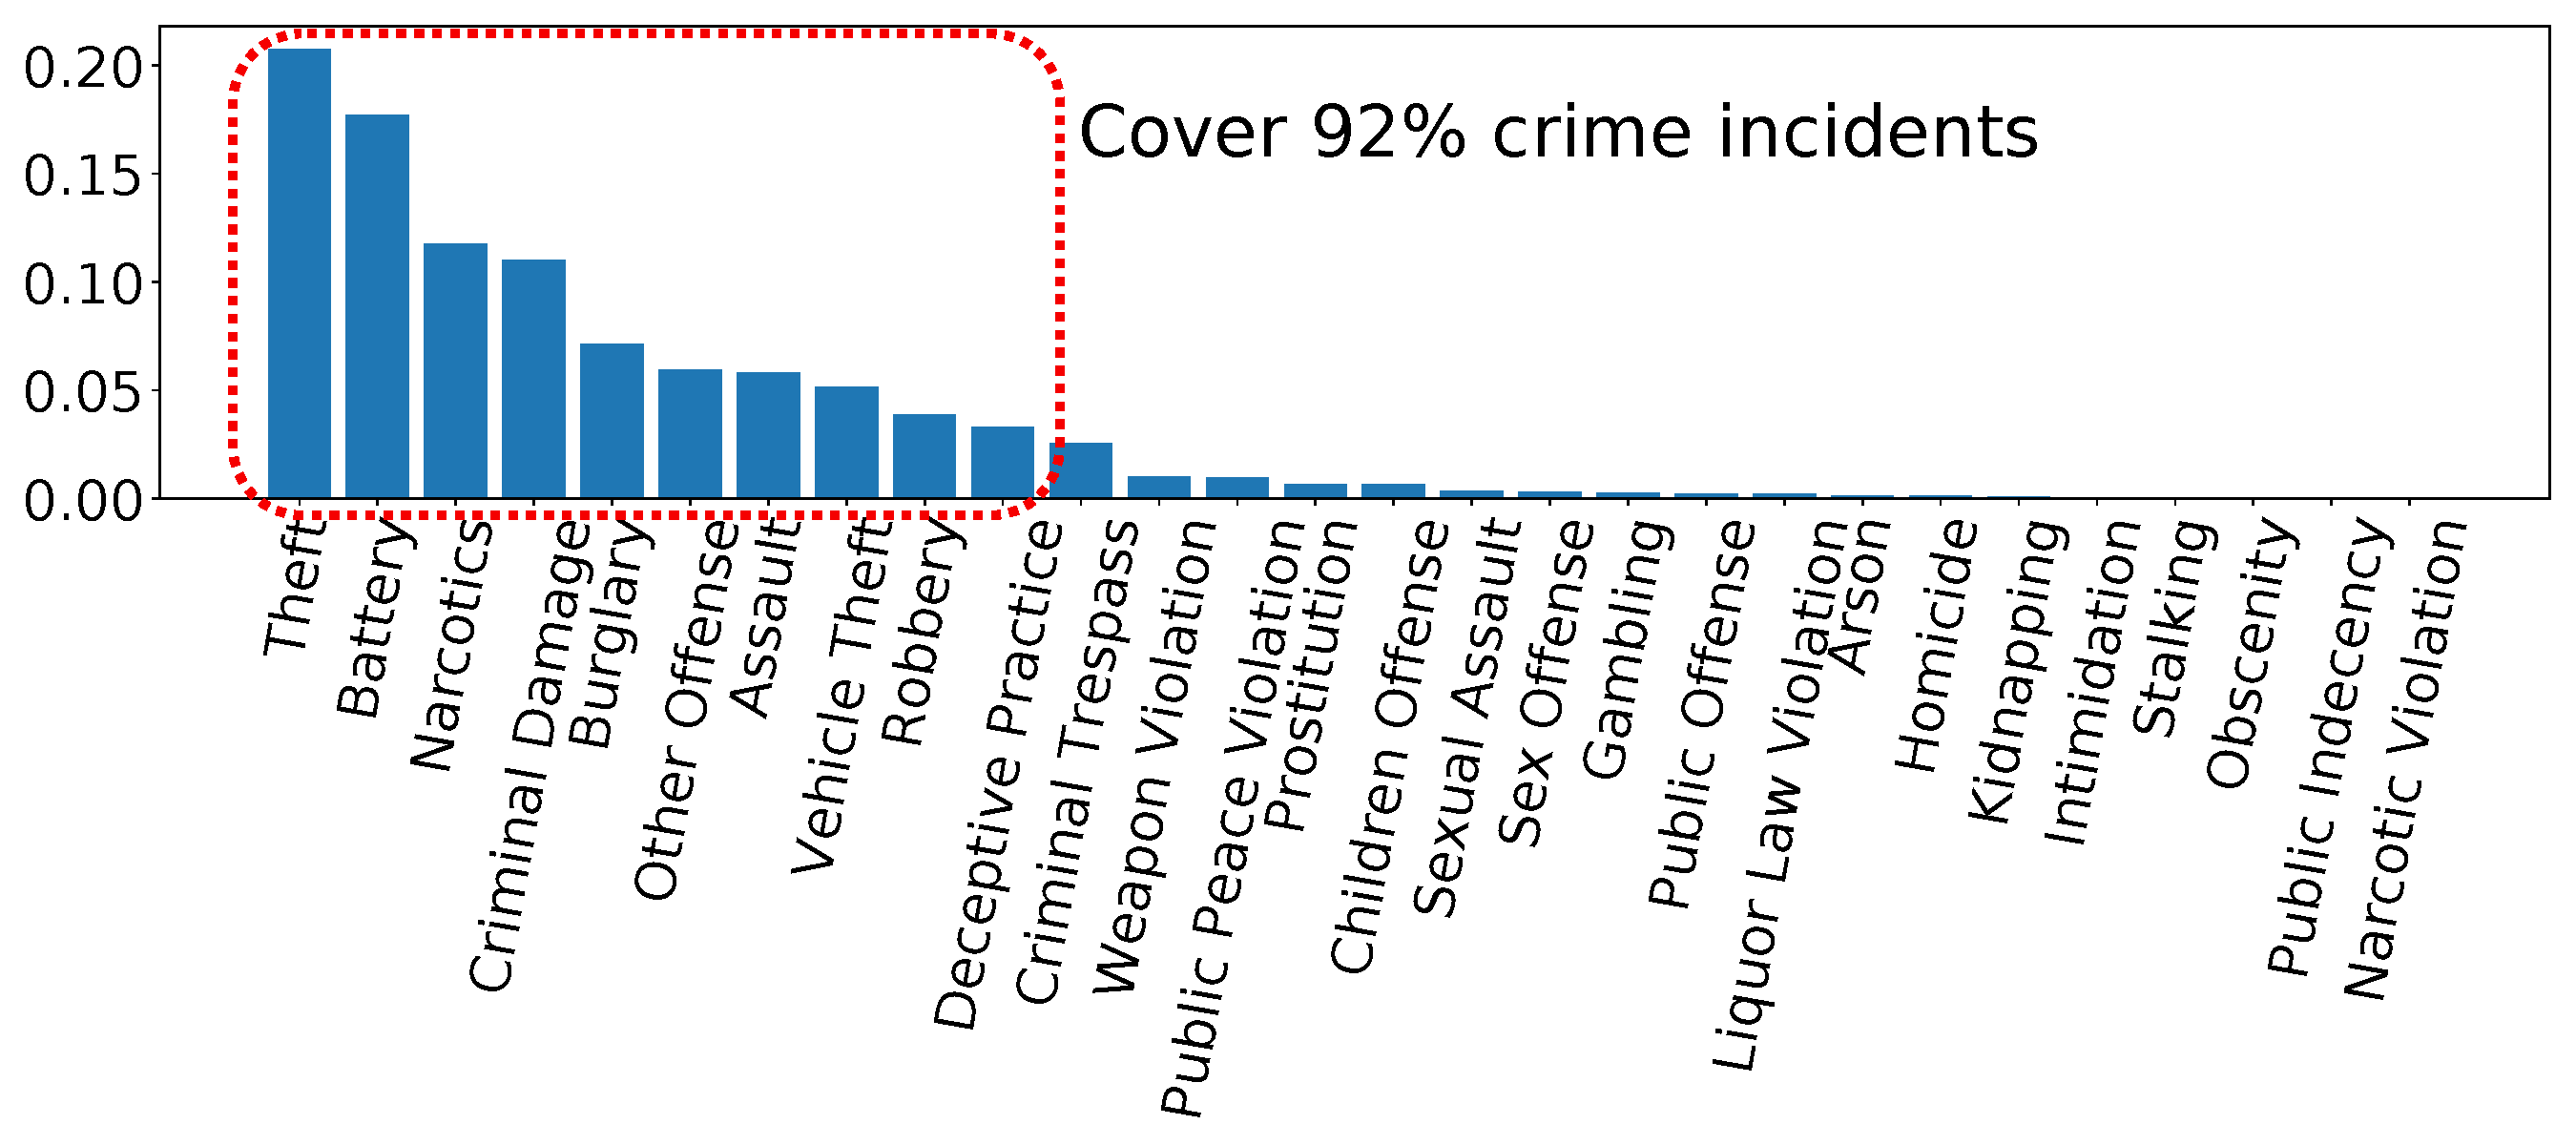
\includegraphics[width=\linewidth]{fig/cate_rate.pdf}
	\caption{Crime rate distribution of different categories in year 2014. Top-10 categories cover 92\% of total crime incidents.}
	\label{fig:cate_rate}
\vspace{-3mm}
\end{figure}


\begin{table}[th]
	\centering
	\caption{Performance of GWNBR on top-10 crime categories in year 2014.}
	\label{tb:categoperf}
	\begin{tabular}{|c|c|c|c|c|c|}
		\hline
		\multicolumn{2}{|c|}{} & \multicolumn{4}{|c|}{Settings} \\ \hline
		\multicolumn{2}{|c|}{Column ID} & 1 & 2 & 3 & 4 \\ \hline
		\multirow{4}{*}{Features}	& \textbf{D}emo & \checkmark& \checkmark& \checkmark& \checkmark \\ \cline{2-6}
		& \textbf{G}eo & \checkmark & \checkmark& \checkmark& \checkmark \\ \cline{2-6}
		& \textbf{P}OI & &\checkmark & & \checkmark \\ \cline{2-6}
		& \textbf{T}axi & & & \checkmark& \checkmark \\ \hline
		Category& Error & \multicolumn{4}{|c|}{} \\ \hline
		\multirow{2}{*}{Theft} & MAE  &  97.64 & \textbf{88.01} & 97.88 & 92.83\\ \cline{2-6}
		& MRE & 0.347 & \textbf{0.313} & 0.348  & 0.330 \\\hline
		\multirow{2}{*}{Battery} & MAE & 59.65 & 57.74 & 59.95 & \textbf{55.30}\\ \cline{2-6}
		& MRE & 0.251 & 0.243 & 0.252 & \textbf{0.232}\\\hline
		\multirow{2}{*}{Narcotics} & MAE &61.58 & 65.05 & \textbf{59.54} & 62.38\\ \cline{2-6}
		& MRE & 0.416 & 0.439 & \textbf{0.402} & 0.421\\ \hline
		\multirow{2}{*}{Criminal Damage} & MAE & 29.37 & 32.65 & \textbf{29.11} & 32.40\\ \cline{2-6}
		& MRE & 0.200 & 0.222 & \textbf{0.198} & 0.221\\\hline
		\multirow{2}{*}{Burglary} & MAE & 21.90 & 23.49 & \textbf{21.79} & 23.13\\ \cline{2-6}
		& MRE & 0.237 & 0.254 & \textbf{0.235} & 0.250\\\hline
		\multirow{2}{*}{Other Offense} & MAE & 19.93 & \textbf{16.68} & 20.20 & 17.03\\ \cline{2-6}
		& MRE & 0.241 & \textbf{0.202} & 0.244 & 0.206\\\hline
		\multirow{2}{*}{Assault} & MAE & 19.48 & 18.37 & 18.93 & \textbf{16.36} \\ \cline{2-6}
		& MRE & 0.240 & 0.226 & 0.233 & \textbf{0.202} \\\hline
		\multirow{2}{*}{Motor Vehicle Theft} & MAE & 19.79 & 21.42 & \textbf{19.60} & 21.61 \\ \cline{2-6}
		& MRE & 0.289 & 0.313 & \textbf{0.286} & 0.316 \\\hline
		\multirow{2}{*}{Robbery} & MAE & \textbf{18.94} & 25.97 & 19.18 & 23.27 \\ \cline{2-6}
		& MRE & \textbf{0.376} & 0.516 & 0.381 & 0.452 \\\hline
		\multirow{2}{*}{Deceptive Practice} & MAE & 19.82 & \textbf{15.15} & 20.12 & 15.19\\ \cline{2-6}
		& MRE & 0.428 & \textbf{0.327} & 0.435 & 0.328\\\hline
	\end{tabular}
\vspace{-3mm}
\end{table}

In Table \ref{tb:categoperf}, we show the performance of GWNBR on the top-$10$ crime categories under various feature settings.  There are some interesting results that are different from the total crime. The main reason is that different crime categories usually have very different spatial distribution. Figure \ref{fig:category-rate} shows the distributions for top-10 categories.
\begin{figure*}
	\centering
	%\subfigure[Total Crime]{\includegraphics[width=0.19\textwidth]{fig/crime_total.pdf}}
	\subfigure[Theft]{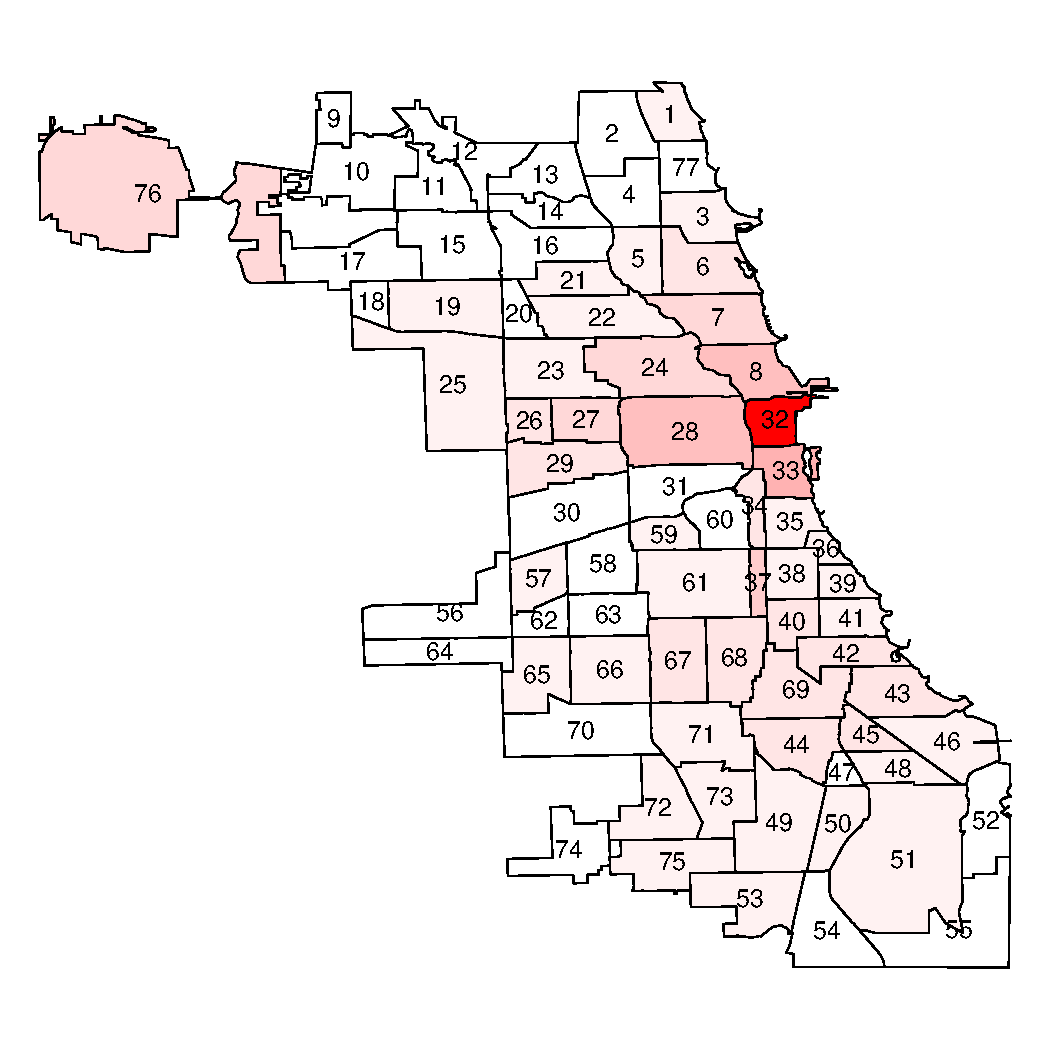
\includegraphics[width=0.24\textwidth]{fig/crime_THEFT.pdf}}
	\subfigure[Battery]{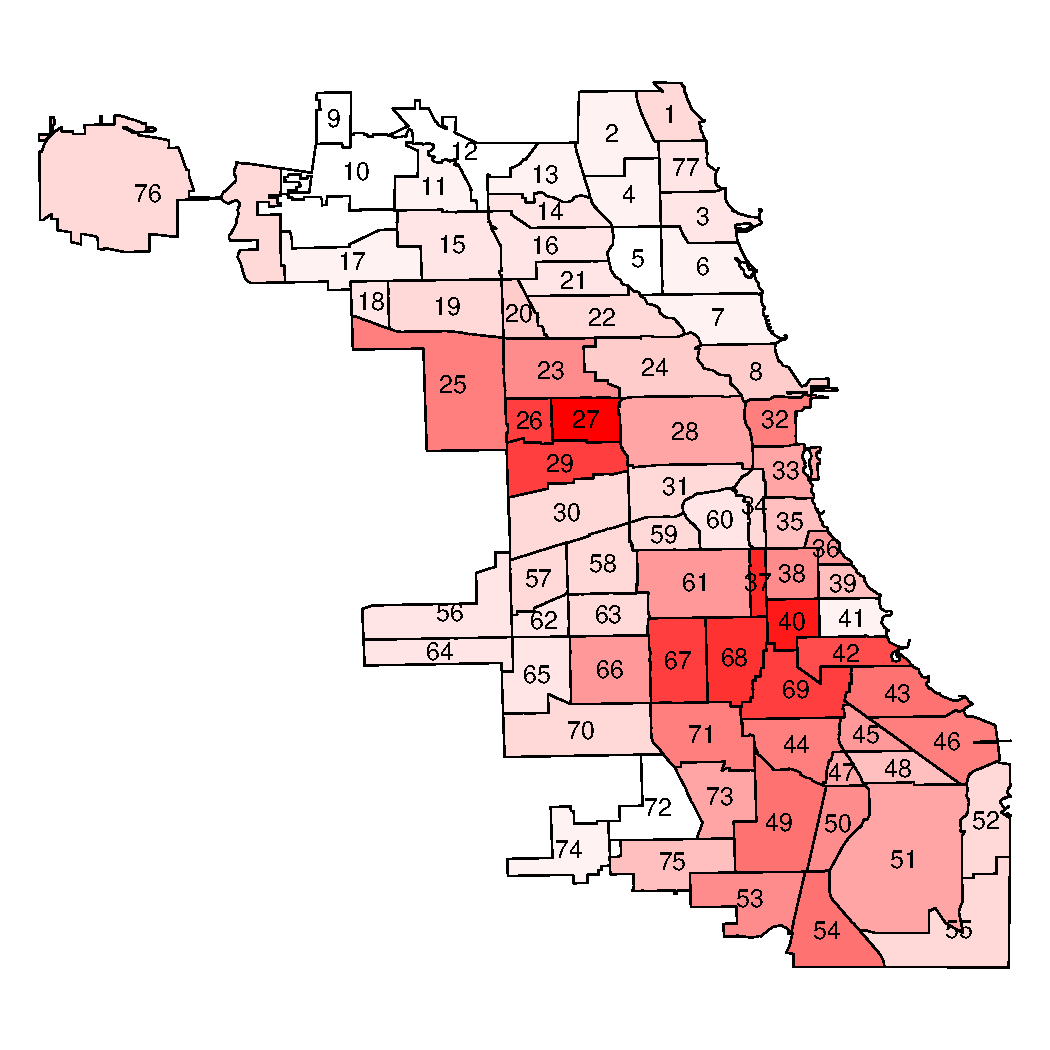
\includegraphics[width=0.24\textwidth]{fig/crime_BATTERY.pdf}}
	\subfigure[Narcotics]{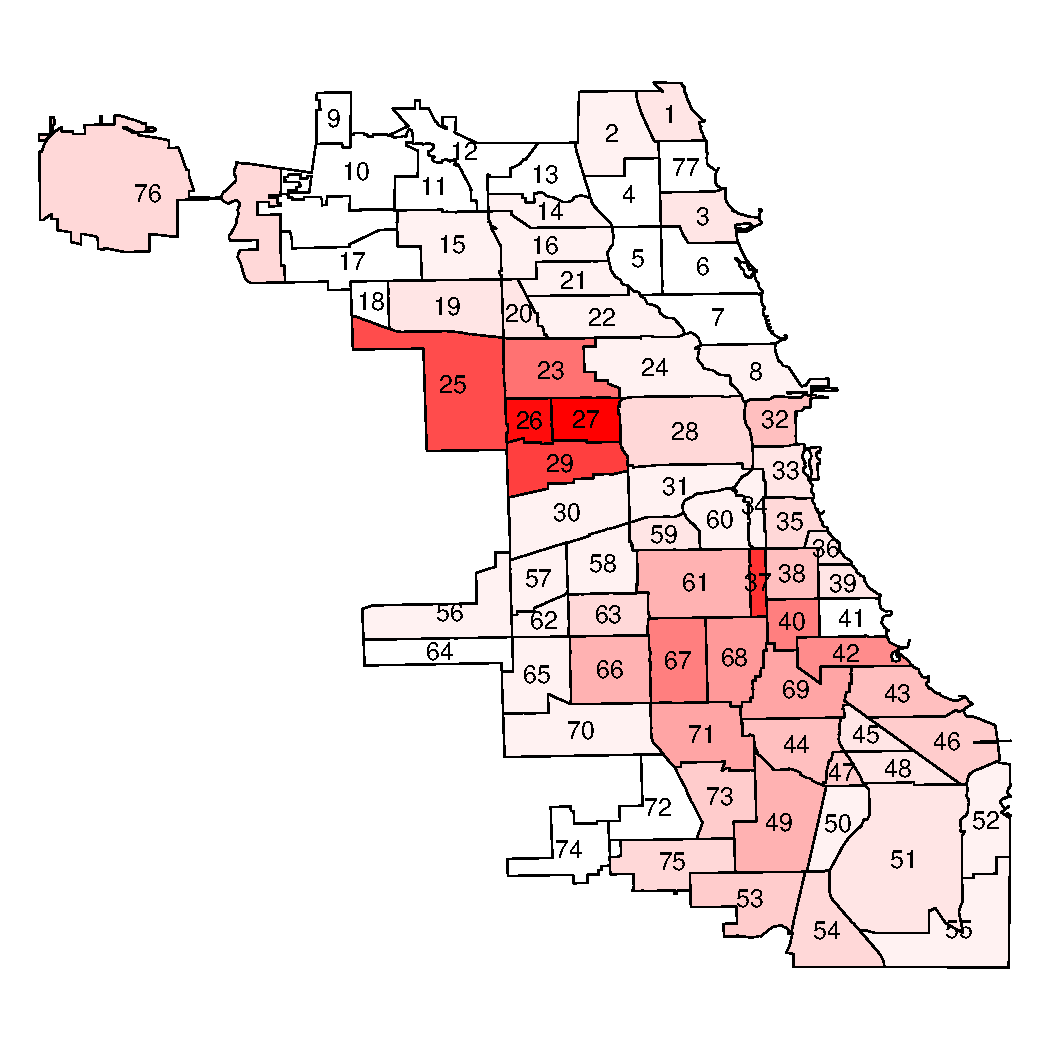
\includegraphics[width=0.24\textwidth]{fig/crime_NARCOTICS.pdf}}
	
	\subfigure[Criminal Damage]{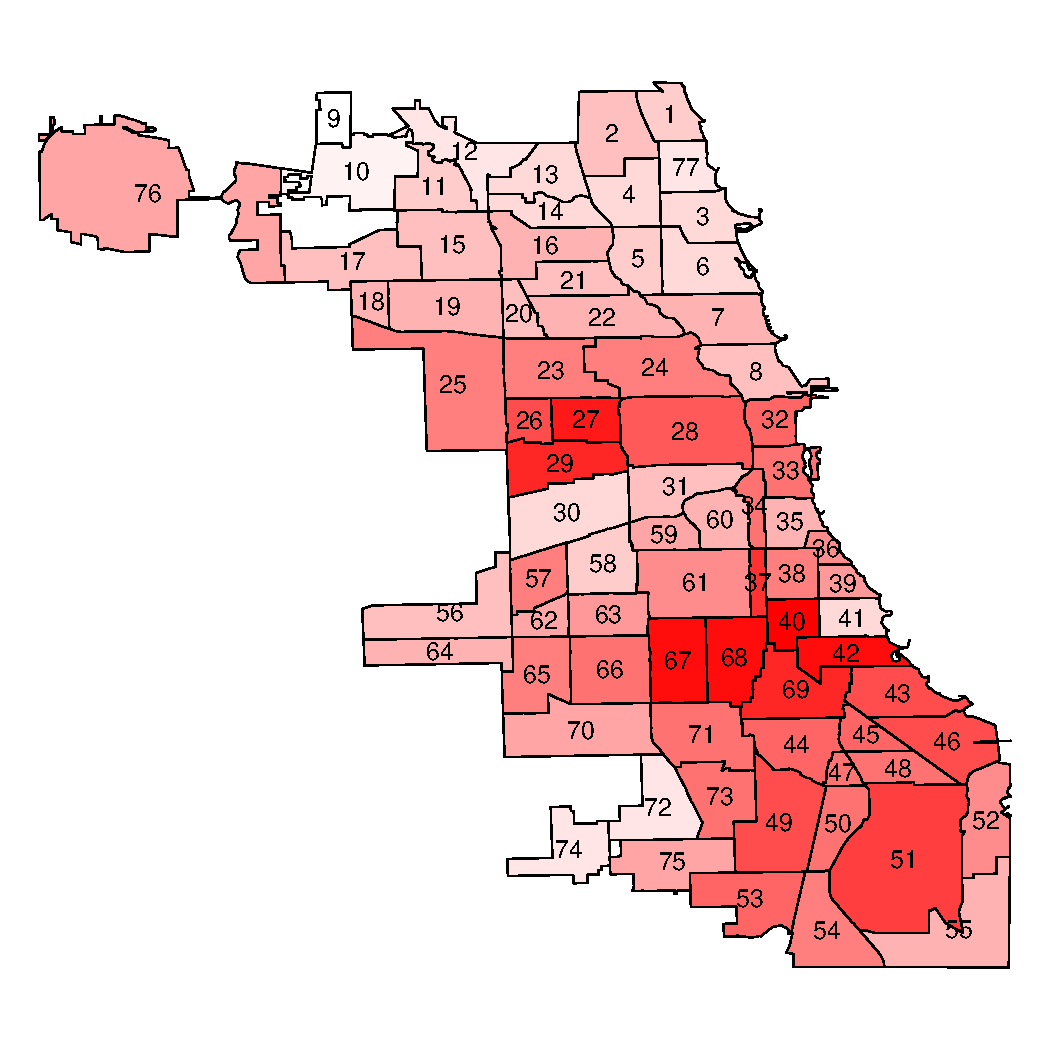
\includegraphics[width=0.24\textwidth]{fig/crime_CRIMINAL_DAMAGE.pdf}}
	\subfigure[Burglary]{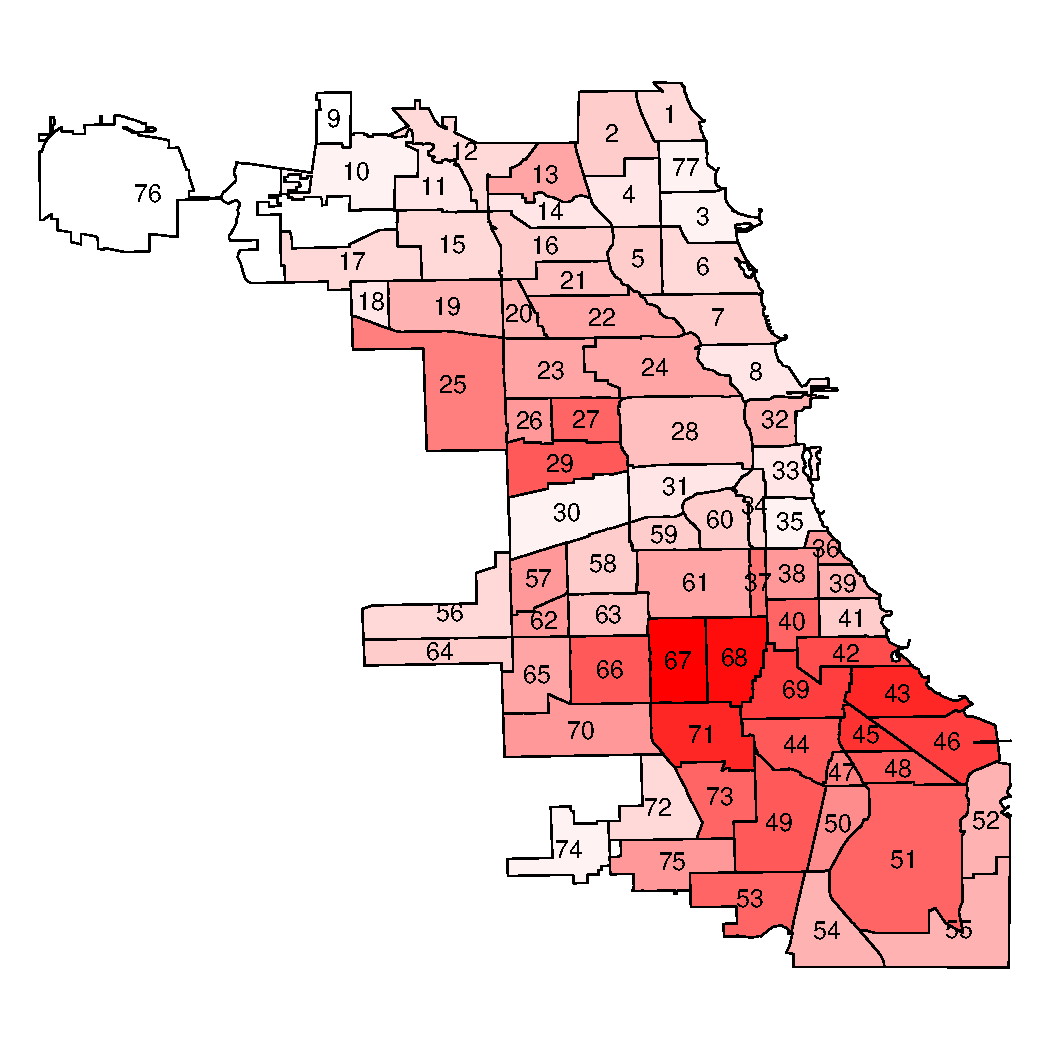
\includegraphics[width=0.24\textwidth]{fig/crime_BURGLARY.pdf}}
	\subfigure[Other Offense]{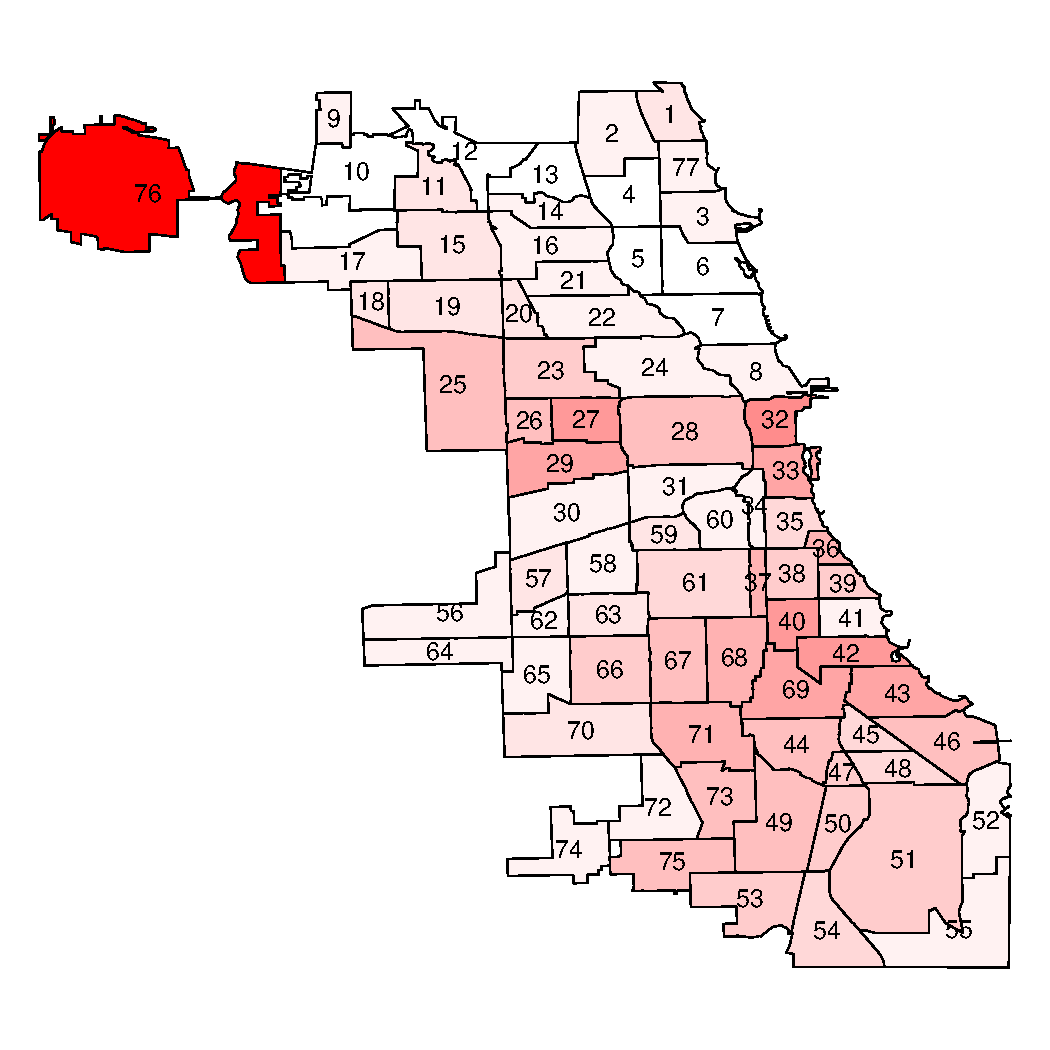
\includegraphics[width=0.24\textwidth]{fig/crime_OTHER_OFFENSE.pdf}}
	
	\subfigure[Assault]{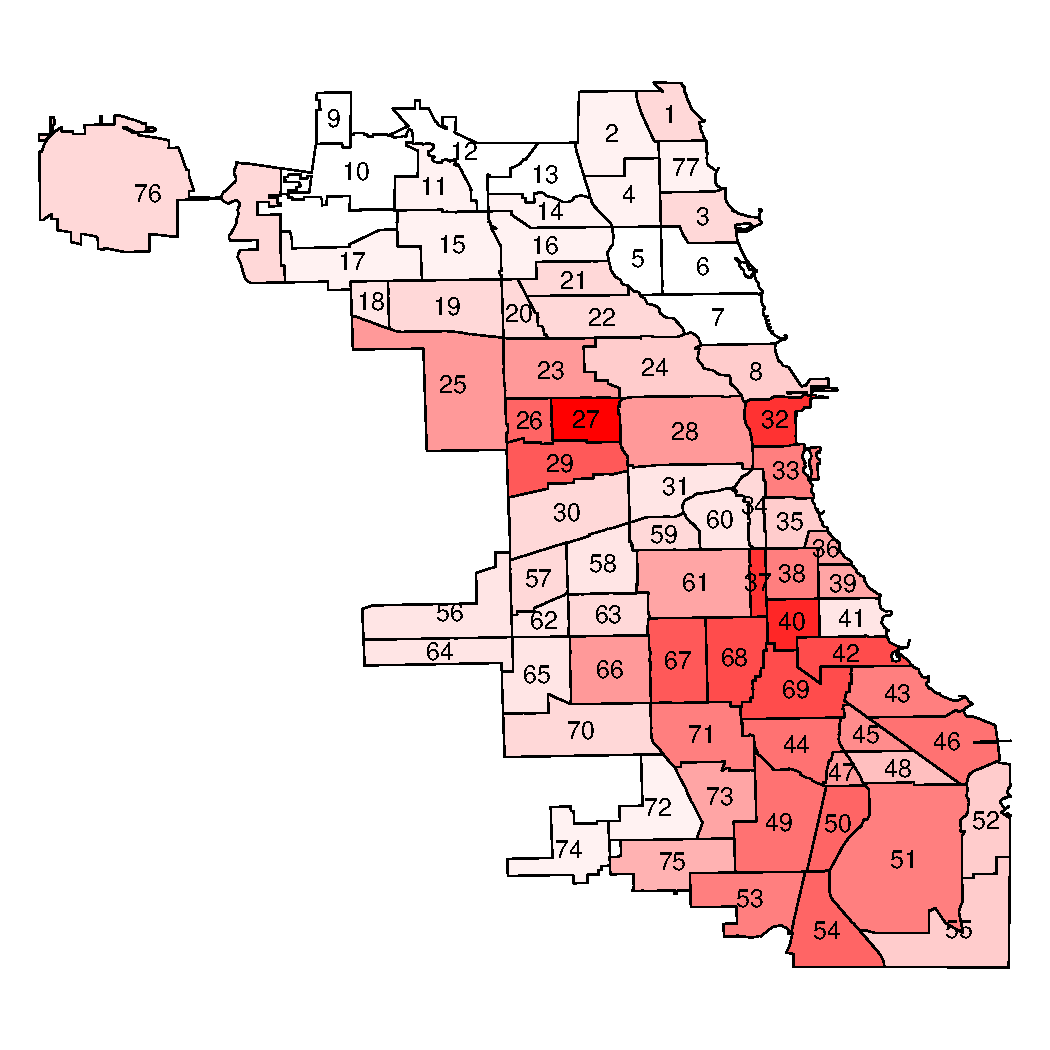
\includegraphics[width=0.24\textwidth]{fig/crime_ASSAULT.pdf}}
	\subfigure[Motor Vehicle Theft]{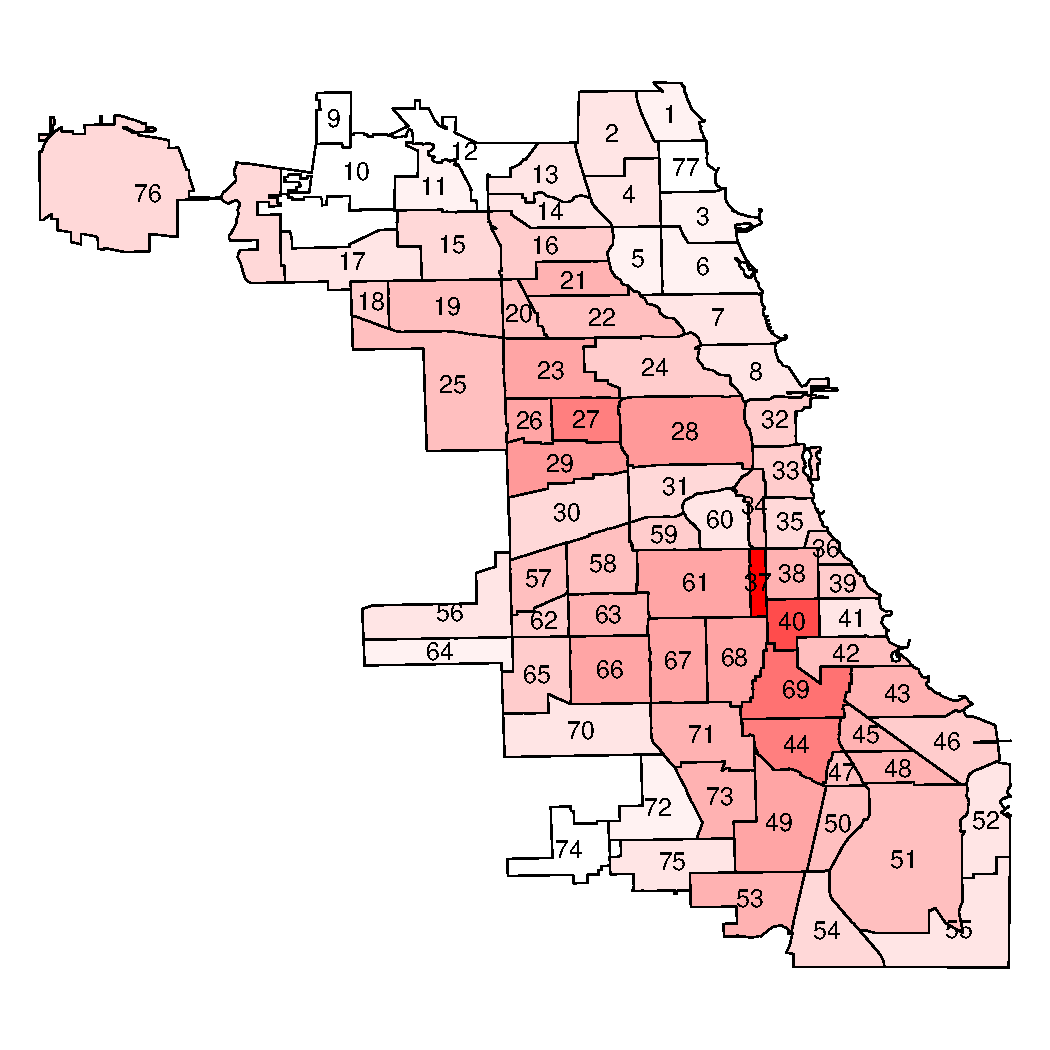
\includegraphics[width=0.24\textwidth]{fig/crime_MOTOR_VEHICLE_THEFT.pdf}}
	\subfigure[Robbery]{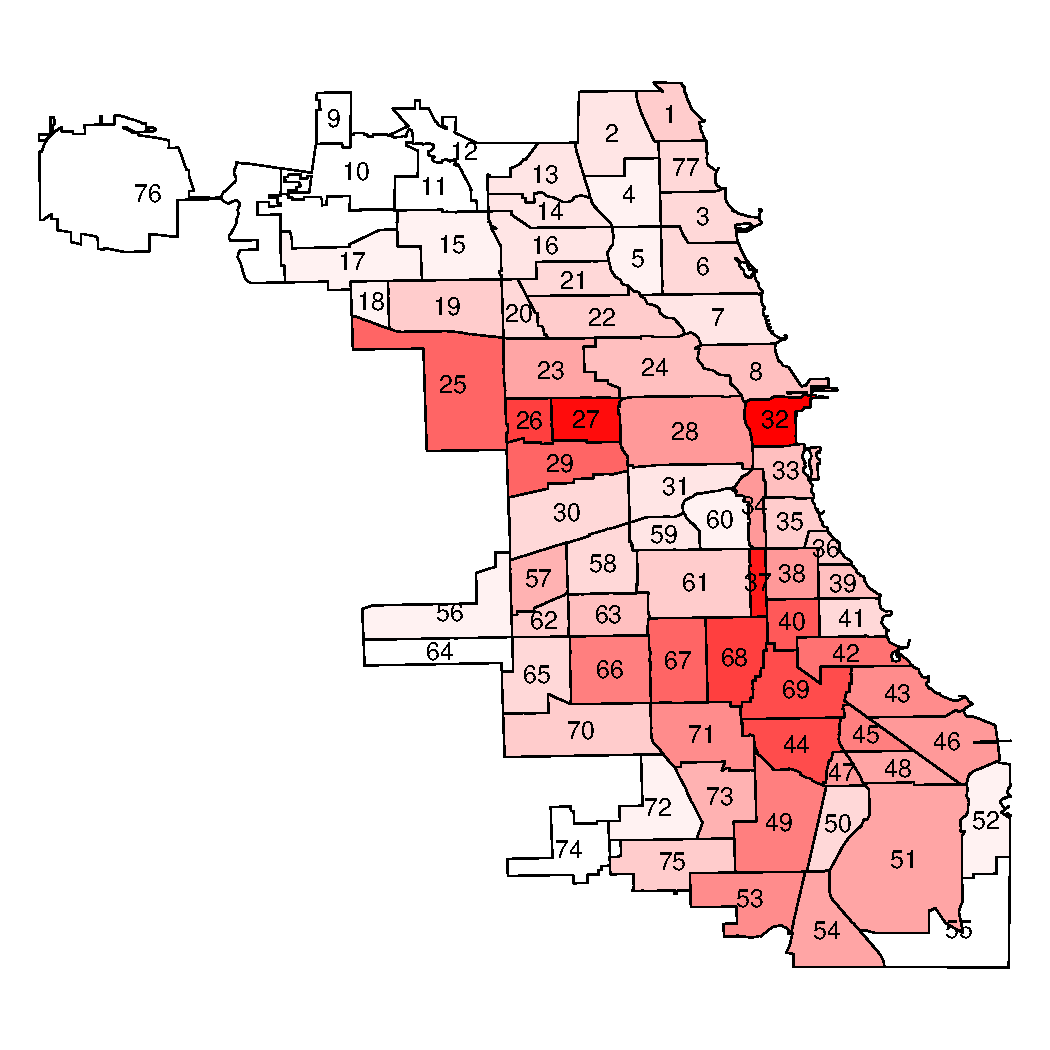
\includegraphics[width=0.24\textwidth]{fig/crime_ROBBERY.pdf}}
	\subfigure[Deceptive Practice]{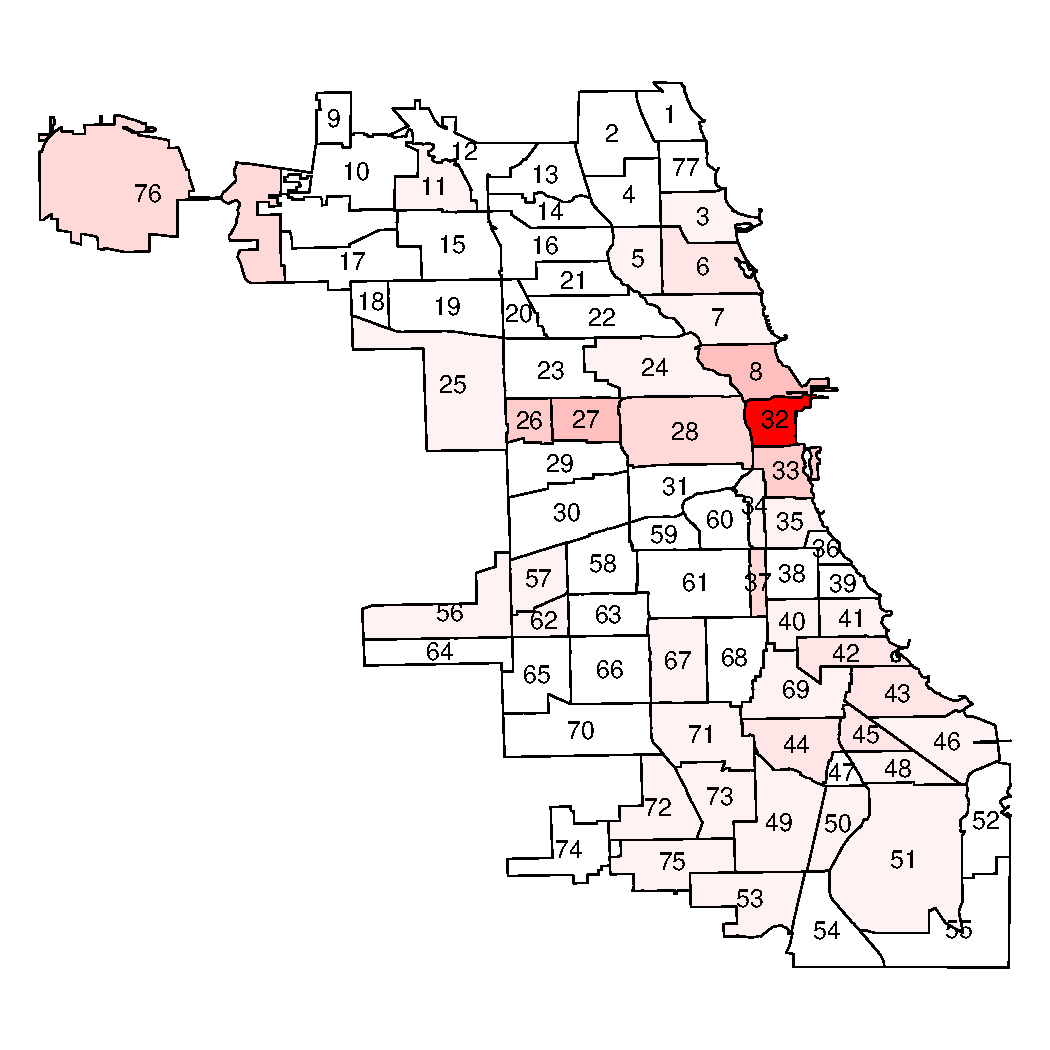
\includegraphics[width=0.24\textwidth]{fig/crime_DECEPTIVE_PRACTICE.pdf}}
	\caption{(a)-(j) Crime rates of overall and top-10 crime categories in Chicago by community areas in year 2014. Darker colors indicate higher values.}
	\label{fig:category-rate}
\vspace{-5mm}
\end{figure*}


\emph{First}, comparing setting 2 to setting 1, POI features make the results worse on the following categories: narcotics, criminal damage, burglary, and motor vehicle theft. From Figure~\ref{fig:category-rate} we can see the distributions of these categories are different from the total crime distribution. The most notable difference is that downtown area is a center for overall crime, but not for these categories. Recall that downtown areas have the highest POIs count from Figure~\ref{fig:poi-dist}. Therefore, the POI features actually correlate less with those categories. In Table~\ref{tb:pairwise_poi}, we quantitatively measure the correlation between crime rate and POI features. Since the POI features are a vector and the crime rate is a scalar, we use a pairwise setting to calculate the correlation. More specifically, we report the Spearman correlation of pairwise difference on crime rates and the pairwise cosine similarity on POI features. The Spearman correlation is typically negative, because if two communities have similar POI distributions (large cosine similarity), then their crime rate difference should be small. Overall, we observe that crime rates in narcotics, criminal damage, burglary, and motor vehicle theft have small or close to 0 correlations with POI distributions.

\emph{Second}, under the theft, deceptive practice, and other offense crime categories, \textbf{D+G+P} (setting 2) achieves the best performance. From Table~\ref{tb:pairwise_poi} we can see that the correlations between POI and crime rate of theft, deceptive practice, and other offense are actually much stronger than other crime categories. The total crime has a correlation of $-0.109$, and all these three categories have much lower correlation values around $-0.2$. This demonstrates that the POI feature is a dominant feature in crime prediction for these three categories. As a result, the \textbf{D+G+P} feature setting has the best performance for these three categories. 

\emph{Third}, under narcotics, criminal damage, burglary, and motor vehicle theft crime categories, \textbf{D+G+T} (setting 3) gives the best performance. These crime categories usually have a high biased distribution toward suburb area according to Figure~\ref{fig:category-rate}. Recall from Figure~\ref{fig:feat-area} that taxi flow helps the most in suburb area, because the social interactions in those areas have a significant influence on crime.


\emph{Fourth}, the robbery is an anomaly category, where neither POI features nor taxi flow features improve the inference accuracy. While this anomaly is hard to explain due to the limitation of our data, we should note that in most cases the POI features and taxi flow features are indeed helpful for crime rate inference. 


\begin{table}
\centering
\caption{Spearman correlation between POI and crime rate. We calculate the correlation in a pairwise setting, because the POI is a vector while the crime rate is a scalar. More specifically, for each pair of regions, we calculate the cosine similarity between their POI features and the difference between their crime rates. Then we report the Spearman correlation of the pairwise difference in crime and the similarity of POI feature. The correlation value is typically negative, indicating that when two communities have similar POI distributions (large cosine similarity), their crime rate difference should be small. For POI performance, ``-'' indicates neutral performance, and ``$\uparrow$'' indicates improved performance.}
\label{tb:pairwise_poi}
\begin{tabular}{|c|c|c|}
  \hline
  Category & Correlation & POI Performance\\\hline
  THEFT & -0.216  & $\uparrow \uparrow$ \\\hline
  BATTERY & -0.103  & $\uparrow$ \\\hline
  NARCOTICS & -0.019 &  -\\\hline
  CRIMINAL DAMAGE & -0.072 &  -\\\hline
  BURGLARY & -0.027 & -\\\hline
  OTHER OFFENSE & -0.226 & $\uparrow \uparrow$ \\\hline
  ASSAULT & -0.145 &  $\uparrow$ \\\hline
  MOTOR VEHICLE THEFT & -0.050 &  -\\\hline
  ROBBERY & -0.077 & - \\\hline
  DECEPTIVE PRACTICE & -0.216 & $\uparrow \uparrow$ \\\hline
  total & -0.109 & $\uparrow$ \\\hline
\end{tabular}
\vspace{-3mm}
\end{table}
